% Please do not change the document class
\documentclass{scrartcl}

% Please do not change these packages
\usepackage[hidelinks]{hyperref}
\usepackage[none]{hyphenat}
\usepackage{setspace}
\doublespace

% You may add additional packages here
\usepackage{amsmath}
\usepackage{graphicx}
\usepackage{wrapfig}
\usepackage[utf8]{inputenc}
\usepackage[english]{babel}
\usepackage[style=ieee]{biblatex}
\usepackage{csquotes}
\graphicspath{{./images/}}
\addbibresource{references.bib}

% Please include a clear, concise, and descriptive title
\title{What are the most important challenges associated with transitioning to Scrum for game development?}

% Please do not change the subtitle
\subtitle{COMP150 - Agile Development Practice}

% Please put your student number in the author field
\author{1804356}

\begin{document}

\maketitle

\begin{abstract}
    Project managers are often tasked with implementing Scrum to teams that are either unfamiliar with or simply against Agile Practices. This paper discusses some of the more common issues raised by teams and supervisors alike and attempts to provide some insight into possible solutions. 
\end{abstract}

\section{Introduction}

  Today's software industry is faced with ever greater challenges, varying from increased pressure on build release frequency all the way to client interaction and feedback. Naturally, the need for new development practices arose and as a consequence more and more companies are transitioning (wholly or partially) to Agile Development Practices \cite{AgileManifesto}, especially Scrum\cite{Scrum, SCRUMProcess}. The purpose of this paper is to identify what the greatest challenges to team productivity are during this very transition period and suggest feasible solutions that can be implemented by project managers to dampen the negative effects the transition can have on a team.
  
 
    \section{Coaching the masses}
    
     Regardless of the degree of transition to Scrum, it is most often the case that teams will encounter several setbacks in the process. In other words, one could state that Tuckman's model of Team Transformation \cite{tuckmanModel} loses its linearity in practical situations \cite{4599458}. 
     
    \subsection{A new mindset}
    
    One of the greatest challenges project managers face when implementing Agile is overwriting the Waterfall mindset of the team with an entirely different one. However, this is no easy task, as it is very common for members of the teams to simply discard the changes or even actively resist the transition \cite{MtnGoat}. This is especially true when dealing with multidisciplinary teams composed of designers, artists, programmers, etc. As it was observed, the issue stems from the fact that the benefits of Agile practices cannot be observed immediately or rather, while the teams agree on their benefits, "the team members develop cold feet when they really had to practice them" \cite{4599456}. It is generally agreed upon that the best course of action in such cases is to implement the practices gradually, in small incremental steps, so team members can familiarize themselves with the new routine \cite{4293601, 4599458, AgileManifesto}. Additionally, any conflicts that arise can be resolved at this stage, before any progress-impeding escalations.
    
    \newpage
    
    \subsection{Productivity impact}
    
    \begin{wrapfigure}{r}{0.55\textwidth}
        \centering
        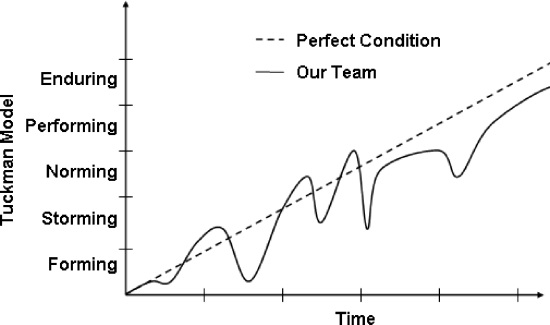
\includegraphics[width=0.45\textwidth]{tuckman.jpg}
        \caption{practice vs. theory}
        \label{fig:tuckman}
    \end{wrapfigure}
    
    As previously stated, the linearity of Tuckman's model of Team Transformation (Figure \ref{fig:tuckman}, \cite{tuckmanModel}) is lost in practice. The reason is that in spite of the team managers' best efforts, teams will inevitably oscillate between different phases. Additionally, it should be noted that the greatest variations are usually encountered during the Storming and the Norming phases (Figure \ref{fig:tuckman}), according to several case studies \cite{4599456, 4599458}. These changes can be attributed to either the team or the project managers pushing for changes that need time to get used to. In other words, the transition period can be considered to be an "experimental" phase in which each team adopts and adapts to changes at its own pace. As it should be expected, some practices prove to be beneficial for the team, while others prove to be detrimental and the team has to roll back the changes. \\
    
    Problems arise, however, when a discrepancy exists between the members of each team, such as, but not limited to: physical location (separate rooms, departments, countries etc.), which in turn leads to the use of web-based meetings, language barriers and even individual personalities (as is the case in most game studios). In such situations, several approaches can be taken: some studies or papers suggest that teams should be encouraged to sort such problems by themselves \cite{4599458, 4599456, 4293601} while others put forward the argument that they should also receive some external guidance (such as taking a gamified\footnote{the application of typical elements of game playing (e.g. point scoring, competition with others, rules of play) to other areas of activity.} approach) to reduce the impact of such conflicts on productivity \cite{7883385, 6475422}, or attempt to adopt new working practices (Such as Clean Code\cite{cleancode}) or improving upon the use of distributed teams. Each of these approaches has been proven to be effective in certain contexts, and therefore project managers should make a decision based on their own circumstances. It should be noted, however, that trial-and-error is likely the best way to find suitable practices\cite{4599458, 4599456, 6475422}.
    
    \section{Evening out}
    
    During the later stages of adopting Agile practices, several papers note the introduction (and the demand for) self-organization within teams \cite{4599458, 4599456, 6986022, 8064437, 6475422}, which can take several forms: leader roles that change by rotation, agile coaching, scrum masters and coordinators. In the case of large scale teams, where Scrums-of-Scrums\cite{Scrum} are implemented, teams will develop their own approach to communicating between each other and will likely require a minimum amount of supervision, while maintaining a certain level of individuality. Project managers should welcome this change and should try to not impose strict limitations on inter-team interaction (such as separation of members or supervision from someone unfamiliar with the team). Another aspect that should be tracked is the addition or removal of team members, which can easily create tensions within the team. Consequently, team composition ought to be well planned and future changes in the team structure, as well as implementing distributed teams, have to be taken into consideration beforehand.
    
    \section{Case study: Guild Wars 2}
    
    During a GDC\footnote{Game Developers Conference} conference in 2016, the developers of the popular MMO\footnote{Massively multiplayer online game} Guild Wars 2, ANet\footnote{Arista Networks, an American-based computer networking company}, held a presentation regarding the challenges encountered during their iterative development process of their latest expansion pack, Heart of Thorns \cite{GW2}. Several challenges are addressed in the presentation such as the number of feedback sources involved in the development loop\cite{AgileManifesto}, the balancing of adding new features and fixing old bugs and adapting the scope of each development loop.
    
    \subsection{Breaking it down}
    
    \begin{wrapfigure}{r}{0.5\textwidth}
        \centering
        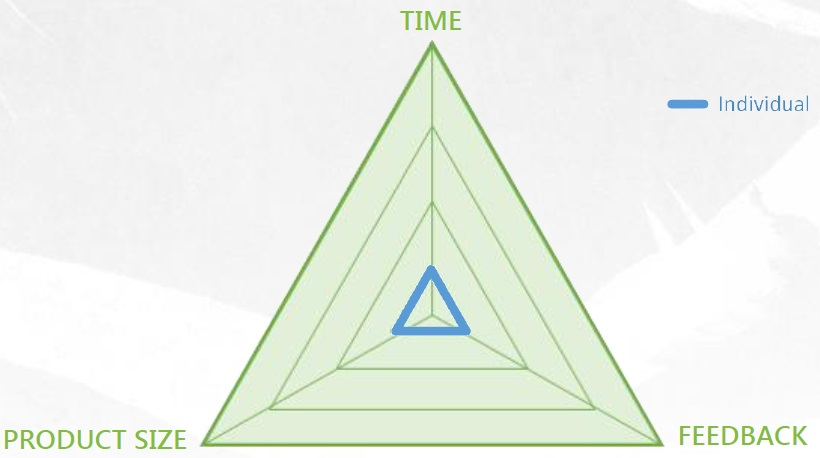
\includegraphics[width=0.5\textwidth]{Loop.jpg}
        \caption{the three levers}
        \label{fig:loop}
    \end{wrapfigure}
    
    The team was able to take an interesting approach to breaking down each development loop (iteration) by breaking it down into 3 "Levers"\cite{GW2} that can be pulled to maximize product value: Time, Product Size and Feedback, as seen in Figure \ref{fig:loop}. This way, each issue can be visualized by scaling each of the levers to represent its nature. This approach is especially effective in pinpointing issues that are hindering progress and encouraging prompt action from the teams.
    
    \subsection{Remarks}
    
    This approach proved to be especially effective in the context of keeping the client(s) involved in the development process, with the number of feedback sources constantly increasing. Furthermore, the team continued to create release versions until the profit margin\footnote{When creating new release versions is deemed unprofitable} was broken, ensuring both a playable (and mostly bug-free) experience, and a time and cost effective product release.
    
    \section{Conclusion}
    
    The author believes that several points can be taken from this paper. In the context of Game Development, where teams often have several specializations (art, design, programming etc.), project managers ought to carefully plan transitioning to Scrum and should not expect said transition to happen overnight. Furthermore, teams should be coached and encouraged to adapt their own version of Agile practices and should be allowed to become more self-driven. Finally, resources for a smoother transition and to encourage the use of Agile practices should always be allocated (co-locating team members, distributed teams, dedicated meeting areas etc.).

\printbibliography

\end{document}
